		\chapter{Fog}
			\textbf{NOTE: This is the entry about Fog that I entered into the Logbook for RCJA Rockhamption Regionals, in July 2015}\\
			
			Experimentation was done in the realm of trying to have fog on stage for added effect. This was never intended to be entered into \index{regionals}regionals, but rather for States and Nationals.	\\				
			
			The first and most obvious is getting a fog machine, however in the rules it states that no mains power will be provided to the dance area. The most obvious solution is to use an inverter on a SLA battery, which is probably the option I'll look at implementing.\\
			
			The other option is by making your own. Generally involves heating up a solution of glycerene and water (fog mixture). I experimented with mixing \index{glycerene}glycerene and water, and heated it - but if anything less fog was produced than just plain water itself. No more work was done on this concept.\\
			
			\textbf{NOTE: I have now obviously created this Fog, and here's some information about how I did it:}\\
			
			I wanted to implement a Fog Machine to add effect for whatever performance I was doing. In the paragraphs above I noted some early attempts on how I wished to achieve this. In the end I settled with borrowing a fog machine from a friend of mine, as well as a 400W \index{inverter}inverter.\\
			
			I attached the fog machine and inverter to a 12V SLA boat battery. I am able to carry this around, set it down behind my stage, and fill the stage with fog.\\
			
			\centerline{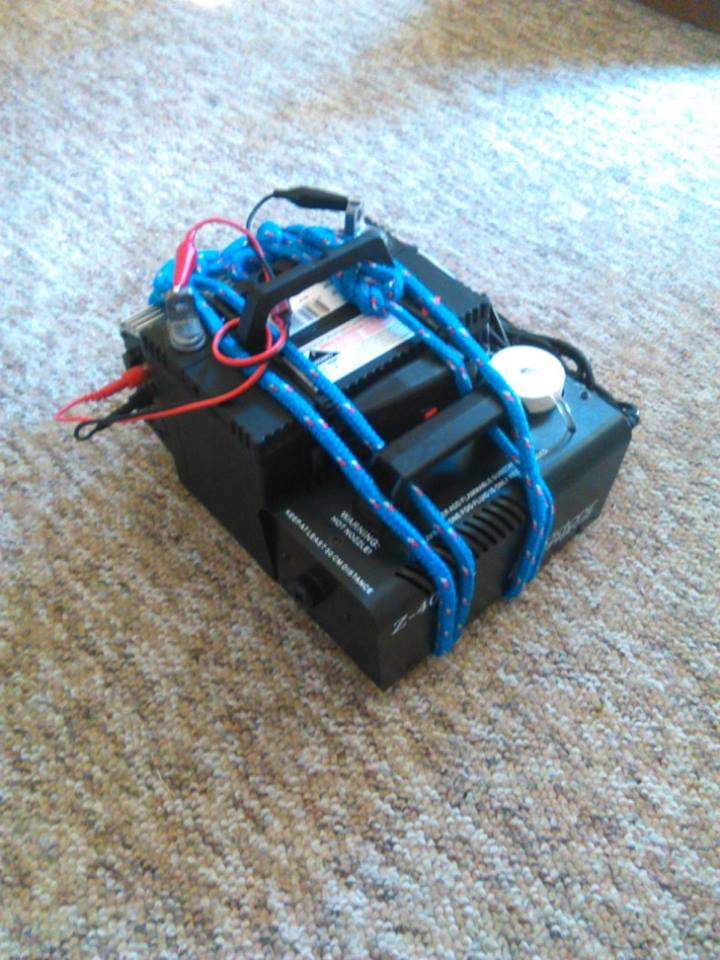
\includegraphics[width=\linewidth]{images/PortaFog}}
			\pagebreak
			
			One problem that I overcame is that the fog machine I borrowed is 400W, and the inverter is also 400W. When turned on the fog machine slightly overloads the inverter - thus shutting the inverter down. If you are unfamiliar with how a fog machine works, it has a heater and a pump. Once the heater has heated, the pump pumps fog "juice" onto the heater, which then evaporates it.\\
			
			The heater draws too much energy for the inverter, but the pump can run off the inverter. What I decided to do was to heat the fog machine up using mains power, and once the heater has heated, I switch it over to inverter power. I am then able to pump fog juice onto the heater, without the heater requiring any energy.\\
			
			After fogging for a set period of time the heater needs to be heated once again - at this point the inverter stalls. I have sufficient time to pump out all the fog I need before the heater has cooled down though.\\
			
			I ran a few experiments testing how long I could use the fog machine before it needed mains power again, and I found that after 2 minutes off mains power (and not being used) the fog machine is able to fog for 26.5 seconds. I feel that 2 minutes is sufficient time for me to unplug the machine, take it to the stage, set up, and start fogging before the heater cools.\\
			
			\centerline{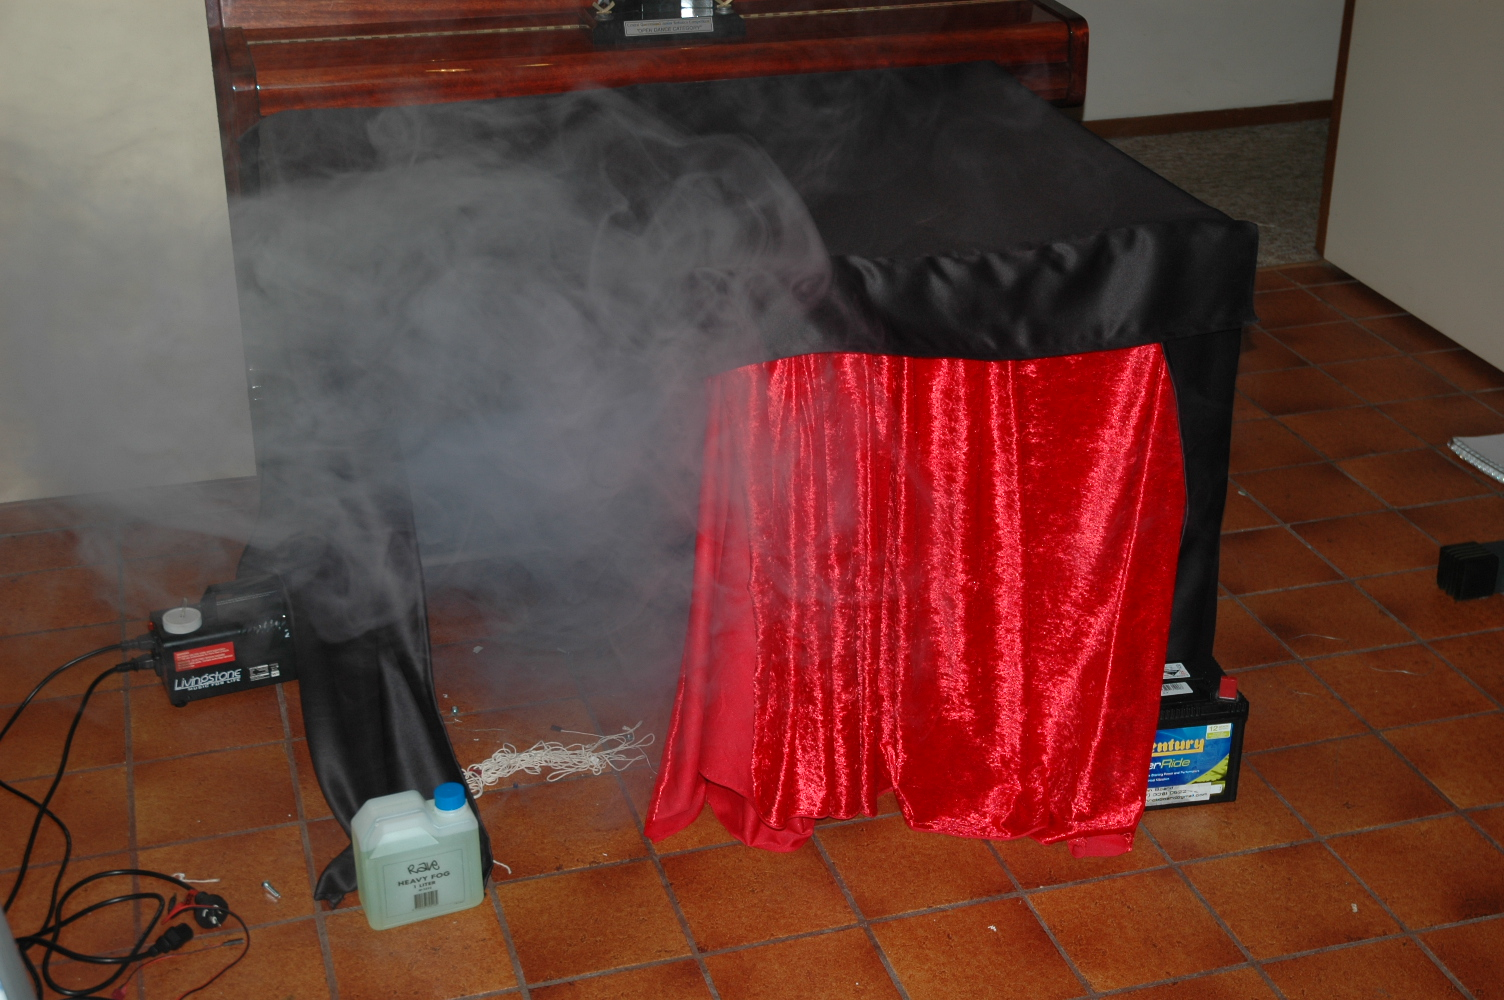
\includegraphics[width=0.75\linewidth]{images/FogTest}}